\documentclass[12pt]{article}

\usepackage{sbc-template}
\usepackage{graphicx,url,hyperref}

\usepackage[brazilian]{babel}
%\usepackage[latin1]{inputenc}
\usepackage[utf8]{inputenc}

\usepackage{listings}
\sloppy

\title{Análise Forense em Pacotes de Dados:\\Captura e Remontagem}

\author{Guilherme de M. M. Taschetto\inst{1}}

\address{Faculdade de Informática -- Pontifícia Universidade \\Católica do Rio Grande do Sul
  (PUCRS)\\Porto Alegre -- RS -- Brazil
}

\begin{document}

\maketitle

\begin{abstract}
  This article presents an introduction to network analysis forensics tools, enlighetning its importance, operation and discurring about its usage implications and results.
\end{abstract}

\begin{resumo}
  Este artigo apresenta uma introdução às ferramentas forenses de análise de rede, salientando a sua importância, a sua forma de funcionamento e discorrendo sobre as implicações do seu uso e de seus resultados.
\end{resumo}

\section{Introdução}

A importância da perícia forense digital cresceu muito nos últimos anos. Através de processos, metodologias e ferramentas, a perícia forense digital é capaz de produzir as evidências e provas necessárias para condenar (ou inocentar) criminosos digitais.

Este artigo estuda um grupo particular de ferramentas: as ferramentas de rede para perícia forense. Tais ferramentas são de muita importância para o processo forense, pois elas coletam dados de todos os ativos disponíveis na rede como: IDS, IPS, Servidor de Logs, conexões capturadas por sniffers de rede etc. Após a coleta de evidências, é necessário realizar a análise destes pacotes. Para isto, são utilizadas as ferramentas de análise forense de redes, onde os pacotes capturados serão usados como base para remontar os dados reais das camadas mais altas de aplicação.

Tais dados ajudam ajudam o perito computacional na obtenção de evidências para solução dos casos, fornecendo provas irrefutáveis que serão apresentadas no laudo pericial.

\section{Ferramentas de Análise Forense de Redes}

Ferramentas de Análise Forense de Redes (Network Forensic Analysis Tool, NFAT) normalmente realizam análises à partir de arquivos PCAP, que pode ser facilmente gerados em aplicações bem conhecidas como Wireshark. Em arquivos PCAP são armazenados fluxos de comunicação de rede de diversos protocolos. Ao analisar estes arquivos, as ferramentas NFAT conseguem extrair os dados das comunicações. Por exemplo:

\begin{itemize}
  \item Requisições e páginas HTML (+JS + CSS) sobre o protocolo HTTP;
  \item E-mails sobre os protocolos POP, SMTP e IMAP;
  \item Conversas telefônicas sobre o protocolo SIP;
  \item Entre diversas outros protocolos de aplicação, como DNS, ARP, SIP, FTP, TFTP etc.
\end{itemize}

Porém não há mágica: não há como remontar os dados trocados em comunicações seguras (criptografadas), porém é possível identificar diversas informações da comunicação em si - por exemplo, endereços físicos e lógicos das partes envolvidas.

Alémd isso é importante salientar que as ferramentas NFAT não são ferramentas de análise e captura de protocolos de rede, e sim ferramentas de análise forense de redes. Embora algumas até possuam o recurso de capturar pacotes, este não é um requisito para considerar a ferramenta NFAT, tampouco é o foco de seus recursos.

\subsection{Xplico}

O Xplico é uma ferramenta NFAT open-source cujo objetivo é extrair dados contidos em arquivos de capturas de pacotes (formato PCAP). O Xplico é distribuído sob a GNU General Public License e alguns scripts sob a Creative Commons Attribution-NonCommercial-ShareAlike 3.0 Unported (CC BY-NC-SA 3.0) License.

As principais características do Xplico são:

\begin{itemize}
  \item Protocolos suportados: HTTP, SMTP, POP, IMAP, SIP, FB, chat, FTP, MSN, IRC, Telnet etc;\footnote{A tabela completa de protocolos suportados pode ser encontrada em http://www.xplico.org/status.}
  \item Identificação de Protocolo Independente de Porta (PIPI) para cada protocolo de aplicação;
  \item Multithreading;
  \item Cada dado remontado pelo Xplico é associado à um arquivo XML contendo todo o fluxo de pacotes correspondentes ao dado remontado;
  \item Remontagem TCP com verificação de ACK para qualquer pacote;
  \item Lookup de DNS reverso;
  \item Sem limite de tamanhos de dados de entrada;
  \item Suporte a IPv4 e IPv6;
  \item Modularidade. Cada componente do Xplico é modular.
\end{itemize}

O Xplico pode ser instalado e executado em qualquer distribuição Linux. Além disso, o projeto hospeda uma versão de demonstração na web suportando arquivos PCAP com no máximo 5 MB. A versão de demonstração pode ser acessada em \href{http://demo.xplico.org/}{http://demo.xplico.org/}.

\subsection{CapAnalysis}

O CapAnalysis é uma ferramenta NFAT web proprietária que também extrai dados à partir de arquivos PCAP. Diferentemente do Xplico, o CapAnalysis proprietário e, portanto, sua licença de uso deve ser paga.

As principais características do CapAnalysis são:

\begin{itemize}
  \item Suporte aos protocolos mais utilizados diariamente no mundo inteiro;
  \item Remontagem TCP;
  \item Filtro avançado de fluxos PCAP;
  \item Inspeção profunda e detalhada de pacotes;
  \item Geolocalização.
\end{itemize}

Assim como o Xplico, o CapAnalysis pode ser instalado e executado em qualquer distribuição Linux. Também conta com uma versão de demonstração online, não informando se há limite para o tamanho do arquivo PCAP. A versão de demonstração pode ser acessada em \href{http://pcap.capanalysis.net/}{http://pcap.capanalysis.net/}.

\section{Estudo de Caso: Xplico}

Como o foco aqui é a análise forense dos pacotes, foi gerado um arquivo PCAP realizando uma captura de alguns segundos através do Wireshark. Durante a captura foram acessadas páginas web não criptografadas, realizadas sincronias utilizando o Dropbox, entre outras operações de rede menos significativas. À partir deste arquivo gerado foi possível extrair diversas informações no Xplico.


\begin{figure}[ht]
    \centering
    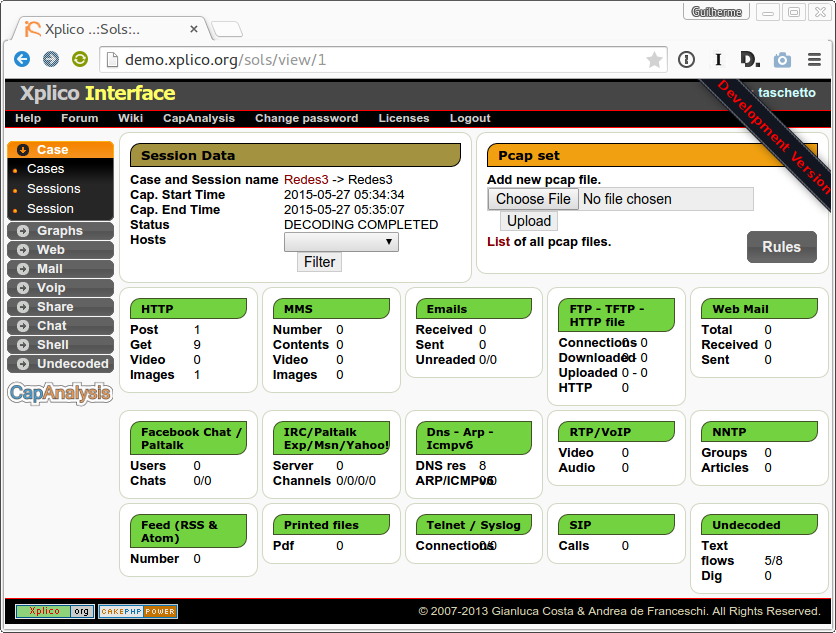
\includegraphics[scale=0.4]{img/2.png}
    \caption{Resumo da Análise}
    \label{fig:report}
\end{figure}

Na figura 1 é apresentado um resumo da análise, com diversas requisições HTTP (tanto GET quanto POST), alguns pacotes DNS e alguns outros que não foram possíveis decifrar (comunicações criptografadas).

\begin{figure}[ht]
    \centering
    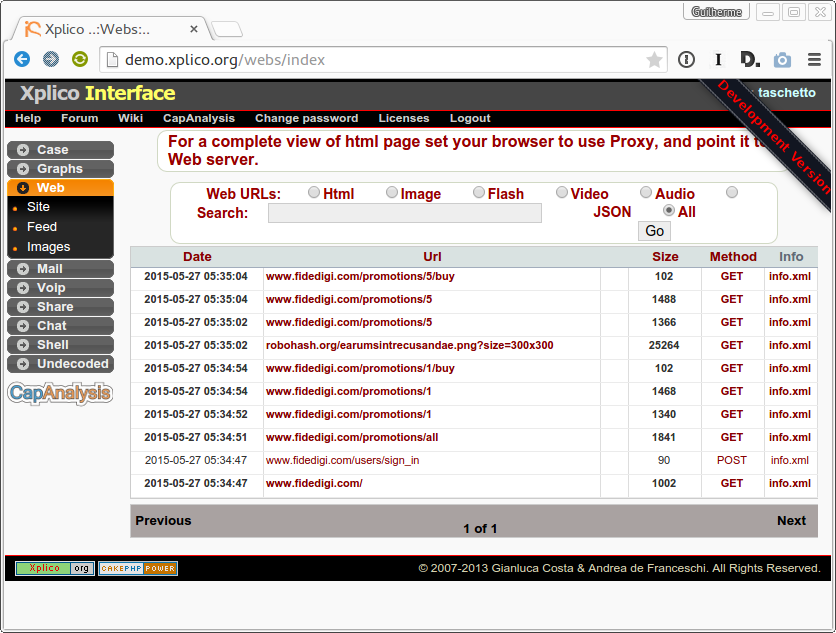
\includegraphics[scale=0.4]{img/1.png}
    \caption{Requisições HTTP}
    \label{fig:http}
\end{figure}

Na figura 2 podemos ver a listagem de todas as requisições HTTP encontradas durante a análise.

\begin{figure}[ht]
    \centering
    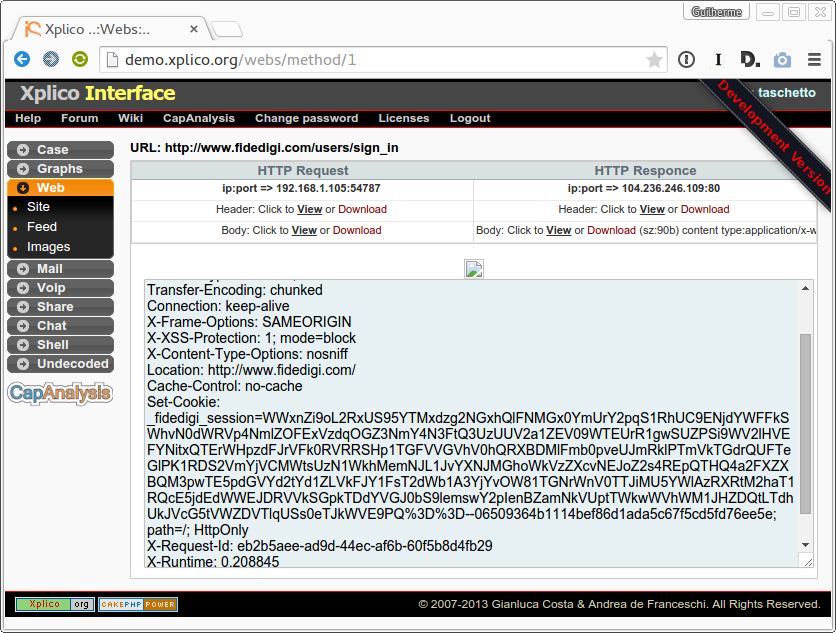
\includegraphics[scale=0.4]{img/3.png}
    \caption{Detalhe do HTTP POST contendo o cookie de sessão}
    \label{fig:cookie}
\end{figure}

Na figura 3 é apresentado o detalhamento dos headers do HTTP POST, contendo uma informação muito interessante: o token de cookie de sessão. Esta informação pode ser utilizada para roubo de sessão, conforme o trabalho do colega William Martins.

\begin{figure}[ht]
    \centering
    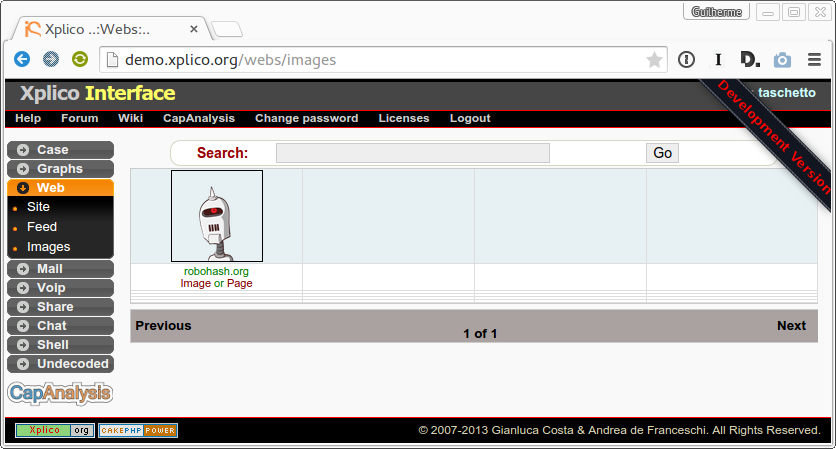
\includegraphics[scale=0.4]{img/4.png}
    \caption{Imagem Recuperada}
    \label{fig:imagem}
\end{figure}

Na figura 4 podemos ver que o Xplico também é capaz de remontar tipos de dados mais complexos, como arquivos de imagem (binário).

\section{Conclusão}

Após a pesquisa e o estudo de ferramentas NFAT, fica evidente a sua relevância e aplicação na computação forense moderna. Executar o Wireshark em modo promíscuo e capturar todo o tráfego de uma rede é uma tarefa trivial. Ser capaz de analisar de forma rápida e simples estes dados capturados é de grande utilidade, seja em investigações públicas como em investigações corporativas. Por exemplo, poder-se-ia identificar usuários acessando conteúdos indevidos na empresa (redes sociais, pornografia, etc) ou até mesmo buscar por consumidores de pedofilia ao analisar o tráfego em pontos estratégicos em WANs.

Entretanto, considero estas ferramentas uma faca de dois gumes: ao mesmo tempo que auxilia na identificação e condenação de infratores e criminosos, também afeta a privacidade dos bons usuários das redes, que não cometem crimes e tem suas informações acessadas muitas vezes sem o seu consentimento.

\bibliographystyle{sbc}
\bibliography{sbc-template}

\end{document}
